\definecolor{r1}{RGB}{86,16,16};
\definecolor{r2}{RGB}{151,28,28};
\definecolor{r3}{RGB}{214,39,40};
\definecolor{r4}{RGB}{227,104,104};
\definecolor{r5}{RGB}{239,169,169};
\definecolor{b1}{RGB}{11,43,65};
\definecolor{b2}{RGB}{22,86,131};
\definecolor{b3}{RGB}{31,119,180};
\definecolor{b4}{RGB}{59,154,222};
\definecolor{b5}{RGB}{124,188,233};
\definecolor{g1}{RGB}{16,60,16};
\definecolor{g2}{RGB}{33,120,33};
\definecolor{g3}{RGB}{49,180,49};
\definecolor{g4}{RGB}{95,211,95};
\definecolor{g5}{RGB}{135,222,135};
\definecolor{p1}{RGB}{39,23,53};
\definecolor{p2}{RGB}{77,47,106};
\definecolor{p3}{RGB}{116,70,160};
\definecolor{p4}{RGB}{148,103,189};
\definecolor{p5}{RGB}{179,149,208};

\definecolor{y1}{RGB}{102,81,0}      
\definecolor{y2}{RGB}{153,122,0}   
\definecolor{y3}{RGB}{255,187,0}    
\definecolor{y4}{RGB}{255,214,102}   
\definecolor{y5}{RGB}{255,239,191}  


\definecolor{tab_orange}{RGB}{255,127,14};
\definecolor{tab_blue}{RGB}{31, 119, 180};
\definecolor{mixed_color}{RGB}{143, 123, 97}
\definecolor{tab_brown}{RGB}{140,86,75};
\definecolor{tab_red}{RGB}{214,39,40}

\usetikzlibrary{decorations.pathreplacing}


\begin{tikzpicture}








\node[inner sep=0pt] (russell) at (10.71,12.92) {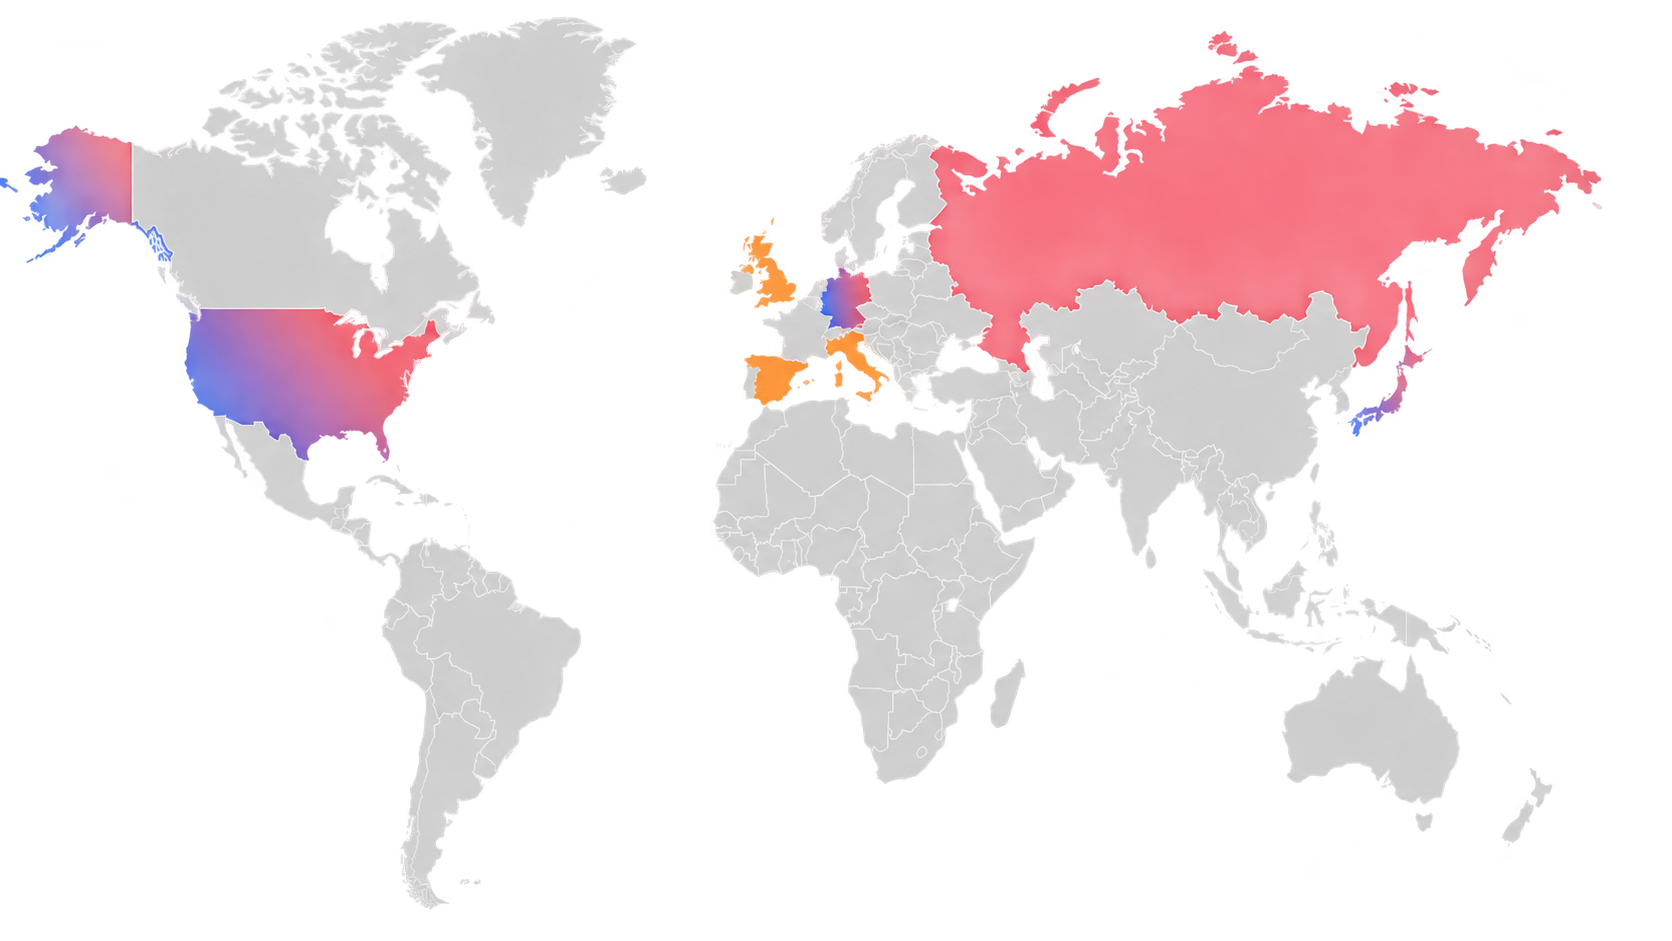
\includegraphics[width=0.3\textwidth]{world.png}};


\node[inner sep=0pt] (russell) at (1.2,9.4) {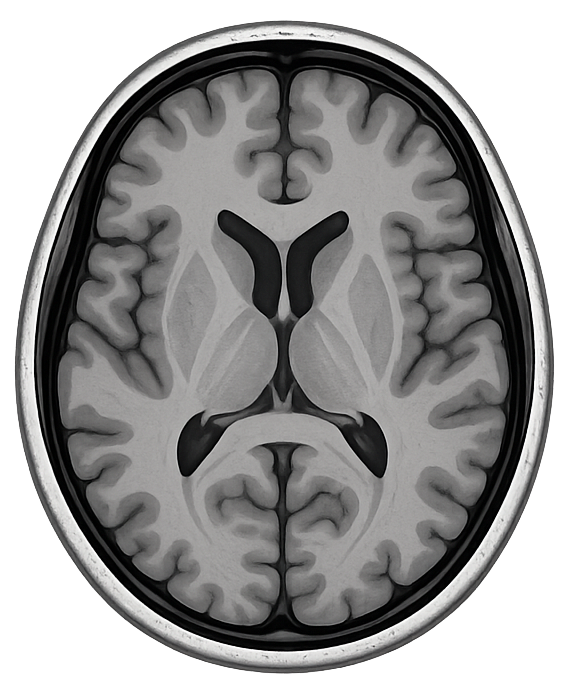
\includegraphics[width=0.04\textwidth]{t1w.png}};
\node[inner sep=0pt] (russell) at (2.3,9) {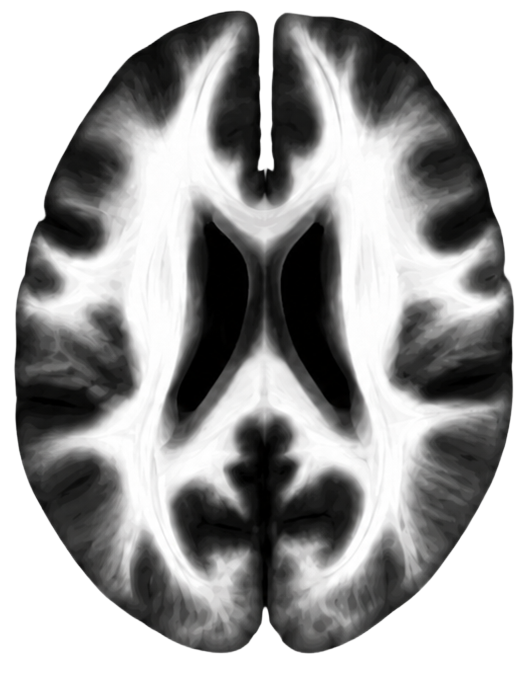
\includegraphics[width=0.02\textwidth]{wmv.png}};
\node[inner sep=0pt] (russell) at (2.3,9.7) {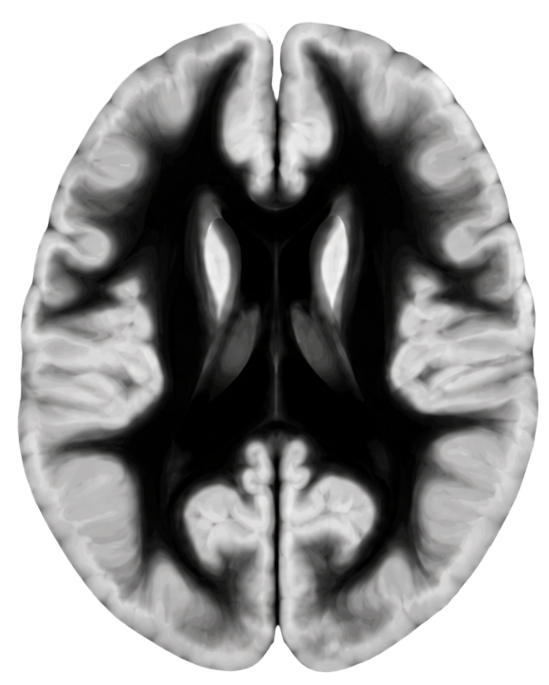
\includegraphics[width=0.02\textwidth]{gmv.png}};
\node[inner sep=0pt] (russell) at (6.9,14) {
\includegraphics[width=0.025\textwidth]{psyshared.png}};

\node[inner sep=0pt] (russell) at (0.9,14) {
\includegraphics[width=0.02\textwidth]{ppnd.pdf}};

\node[inner sep=0pt] (russell) at (5.4,12.91) {
\includegraphics[width=0.02\textwidth]{people1.png}};
\node[inner sep=0pt] (russell) at (1.7,12.91) {
\includegraphics[width=0.02\textwidth]{people2.png}};
\node[inner sep=0pt] (russell) at (2.9,12.91) {
\includegraphics[width=0.02\textwidth]{people3.png}};




\node[inner sep=0pt] (russell) at (2.7,11.9) {
\includegraphics[width=0.01\textwidth]{people1.png}};
\node[inner sep=0pt] (russell) at (1.2,11.9) {
\includegraphics[width=0.01\textwidth]{people2.png}};
\node[inner sep=0pt] (russell) at (2.4,11.9) {
\includegraphics[width=0.01\textwidth]{people3.png}};


\node[inner sep=0pt] (russell) at (2.4,11.5) {
\includegraphics[width=0.01\textwidth]{people1.png}};
\node[inner sep=0pt] (russell) at (2.7,11.5) {
\includegraphics[width=0.01\textwidth]{people2.png}};
\node[inner sep=0pt] (russell) at (1.2,11.5) {
\includegraphics[width=0.01\textwidth]{people3.png}};
\node[inner sep=0pt] (russell) at (1.2,11.7) {
\includegraphics[width=0.01\textwidth]{people1.png}};
\node[inner sep=0pt] (russell) at (2.4,11.7) {
\includegraphics[width=0.01\textwidth]{people2.png}};
\node[inner sep=0pt] (russell) at (2.7,11.7) {
\includegraphics[width=0.01\textwidth]{people3.png}};


\draw  [line width = 0.1mm, rounded corners=1pt]  (0.5,14.5) rectangle (7.4,11.1);
\fill  [gray, opacity=0.1, rounded corners=1pt]  (0.5,14.5) rectangle (7.4,11.1);





\draw  [line width = 0.1mm, rounded corners=1pt]  (0.5,10.7) rectangle (7.4,8);
\fill  [gray, opacity=0.1, rounded corners=1pt]  (0.5,10.7) rectangle (7.4,8);

\node at (2.1,10.8) {{\fontfamily{phv}\scalebox{1}{\fontsize{5pt}{0pt}\selectfont \parbox{3cm} {\textit{Modelling pipeline}}}}};
\node at (9.2,10.8) {{\fontfamily{phv}\scalebox{1}{\fontsize{5pt}{0pt}\selectfont \parbox{3cm} {\textit{Leave cohort out cross-validation}}}}};

























































\node at (2.3,14.1) {{\fontfamily{phv}\scalebox{1}{\fontsize{6pt}{0pt}\selectfont{PPND DataBank}}}};
\node  at (5.4,14.1) {{\fontfamily{phv}\scalebox{1}{\fontsize{6pt}{0pt}\selectfont{Psy-ShareD DataBank}}}};


 
\node  at (8.61,13.3) {{\fontfamily{phv}\scalebox{1}{\fontsize{5pt}{0pt}\selectfont{USA}}}};







\node  at (1.7,13.31) {{\fontfamily{phv}\scalebox{1}{\fontsize{5pt}{0pt}\selectfont{±DEP SSD}}}};
\node  at (2.9,13.31) {{\fontfamily{phv}\scalebox{1}{\fontsize{5pt}{0pt}\selectfont{MDD v HC}}}};

\node  at (5.1,9.7) {{\fontfamily{phv}\scalebox{1}{\fontsize{5pt}{0pt}\selectfont{Base SVM}}}};

\node  at (6.6,9.3) {{\fontfamily{phv}\scalebox{1}{\fontsize{5pt}{0pt}\selectfont{Meta SVM}}}};
\node  at (5.4,13.31) {{\fontfamily{phv}\scalebox{1}{\fontsize{5pt}{0pt}\selectfont{±DEP SSD}}}};
\node  at (6.6,8.5) {{\fontfamily{phv}\scalebox{1}{\fontsize{5pt}{0pt}\selectfont{Predictions}}}};

\node  at (5.1,9) {{\fontfamily{phv}\scalebox{1}{\fontsize{5pt}{0pt}\selectfont{Base SVM}}}};

\node  at (10.2,13.72) {{\fontfamily{phv}\scalebox{1}{\fontsize{5pt}{0pt}\selectfont{UK}}}};


\node  at (10.13,13.22) {{\fontfamily{phv}\scalebox{1}{\fontsize{5pt}{0pt}\selectfont{Spain}}}};



\node  at (10.83,13.92) {{\fontfamily{phv}\scalebox{1}{\fontsize{5pt}{0pt}\selectfont{Germany}}}};



\node  at (11.01,13.02) {{\fontfamily{phv}\scalebox{1}{\fontsize{5pt}{0pt}\selectfont{Italy}}}};


\node  at (1.2,10.2) {{\fontfamily{phv}\scalebox{1}{\fontsize{5pt}{0pt}\selectfont{T1w images}}}};
\node  at (2.3,8.5) {{\fontfamily{phv}\scalebox{1}{\fontsize{5pt}{0pt}\selectfont{WMV maps}}}};
\node  at (2.3,10.2) {{\fontfamily{phv}\scalebox{1}{\fontsize{5pt}{0pt}\selectfont{GMV maps}}}};

\node  at (12.31,13.92) {{\fontfamily{phv}\scalebox{1}{\fontsize{5pt}{0pt}\selectfont{Russia}}}};

\node  at (1.56,8.7) {{\fontfamily{phv}\scalebox{1}{\fontsize{4pt}{0pt}\selectfont{VBM processing}}}};
\node  at (1.2,12.2) {{\fontfamily{phv}\scalebox{1}{\fontsize{4pt}{0pt}\selectfont{Trained on}}}};
\node  at (2.55,12.2) {{\fontfamily{phv}\scalebox{1}{\fontsize{4pt}{0pt}\selectfont{Externally validated on}}}};
\node  at (5.5,12.4) {{\fontfamily{phv}\scalebox{1}{\fontsize{4pt}{0pt}\selectfont{Agreement of predictive patterns}}}};

\node  at (5.1,8.6) {{\fontfamily{phv}\scalebox{1}{\fontsize{4pt}{0pt}\selectfont{Stacked generalisation}}}};
\node  at (3.5,8.5) {{\fontfamily{phv}\scalebox{1}{\fontsize{4pt}{0pt}\selectfont{Preprocessing}}}};

\node  at (13.01,12.92) {{\fontfamily{phv}\scalebox{1}{\fontsize{5pt}{0pt}\selectfont{Japan}}}};









\node at (11.91,11.62) {{\fontfamily{phv}\scalebox{1}{\fontsize{5pt}{0pt}\selectfont \parbox{5cm} {\hyphenpenalty=10000\exhyphenpenalty=10000\raggedright
\textcolor{tab_blue}{\textbf{PPND SSD}}: 8 cohorts, 495 participants
}}}};

\node at (11.91,11.4) {{\fontfamily{phv}\scalebox{1}{\fontsize{5pt}{0pt}\selectfont \parbox{5cm} {\hyphenpenalty=10000\exhyphenpenalty=10000\raggedright
\textcolor{tab_orange}{\textbf{Psy-ShareD SSD}}: 10 cohorts, 279 participants
}}}};


\node at (11.91,11.18) {{\fontfamily{phv}\scalebox{1}{\fontsize{5pt}{0pt}\selectfont \parbox{5cm} {\hyphenpenalty=10000\exhyphenpenalty=10000\raggedright
\textcolor{tab_red}{\textbf{PPND MDD v HC}}: 6 cohorts, 2034 participants
}}}};






\draw  [line width = 0.1mm, rounded corners=1pt]  (4.5,9.9) rectangle (5.7,9.5);
\fill  [b3, opacity=0.25, rounded corners=1pt]  (4.5,9.9) rectangle (5.7,9.5);

\draw  [line width = 0.1mm, rounded corners=1pt]  (4.5,9.2) rectangle (5.7,8.8);
\fill  [b3, opacity=0.25, rounded corners=1pt]  (4.5,9.2) rectangle (5.7,8.8);

\node at (2.1,14.6) {{\fontfamily{phv}\scalebox{1}{\fontsize{5pt}{0pt}\selectfont \parbox{3cm} {\textit{Study design}}}}};

















\node[inner sep=0pt] (russell) at (6.6,9.9) {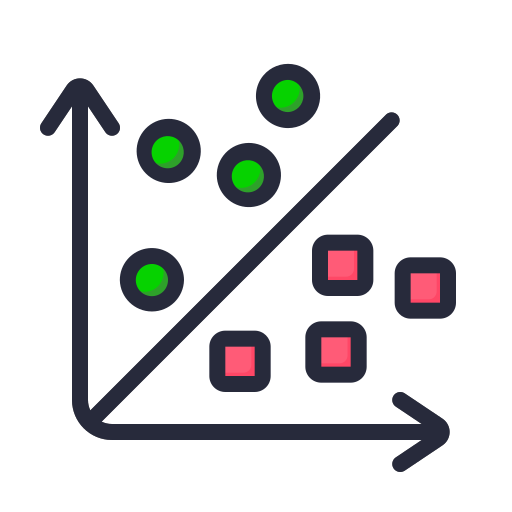
\includegraphics[width=0.025\textwidth]{classification.png}};


\node[inner sep=0pt] (russell) at (5.1,10.2) {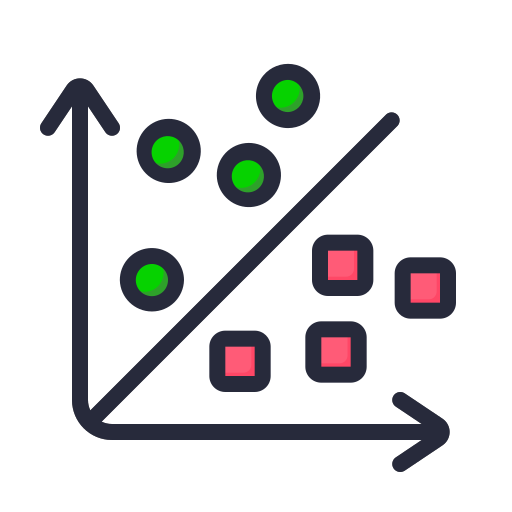
\includegraphics[width=0.025\textwidth]{classification.png}};




\node  [outer sep=0,inner sep=0,minimum size=0] (v1) at (2.3,13.9) {};
\node  [outer sep=0,inner sep=0,minimum size=0] (v2) at (2.9,13.5) {};
\draw  [->, line width = 0.25mm, tab_blue](v1) edge (v2);

\node  [outer sep=0,inner sep=0,minimum size=0] (v1) at (2.3,13.9) {};
\node  [outer sep=0,inner sep=0,minimum size=0] (v2) at (1.7,13.5) {};
\draw  [->, line width = 0.25mm, tab_blue](v1) edge (v2);

\node  [outer sep=0,inner sep=0,minimum size=0] (v1) at (5.4,13.9) {};
\node  [outer sep=0,inner sep=0,minimum size=0] (v2) at (5.4,13.5) {};
\draw  [->, line width = 0.25mm, tab_blue](v1) edge (v2);

\node  [outer sep=0,inner sep=0,minimum size=0] (v1) at (1.5,11.9) {};
\node  [outer sep=0,inner sep=0,minimum size=0] (v2) at (2.1,11.9) {};
\draw  [->, line width = 0.25mm, tab_blue](v1) edge (v2);

\node  [outer sep=0,inner sep=0,minimum size=0] (v1) at (1.5,11.5) {};
\node  [outer sep=0,inner sep=0,minimum size=0] (v2) at (2.1,11.5) {};
\draw  [->, line width = 0.25mm, tab_blue](v1) edge (v2);

\node  [outer sep=0,inner sep=0,minimum size=0] (v1) at (1.5,11.7) {};
\node  [outer sep=0,inner sep=0,minimum size=0] (v2) at (2.1,11.7) {};
\draw  [->, line width = 0.25mm, tab_blue](v1) edge (v2);

\draw  [->, line width = 0.25mm, tab_blue](v1) edge (v2);


\node  [outer sep=0,inner sep=0,minimum size=0] (v1) at (1.7,9.4) {};
\node  [outer sep=0,inner sep=0,minimum size=0] (v2) at (2.1,9.7) {};
\draw  [->, line width = 0.25mm, tab_blue](v1) edge (v2);

\node  [outer sep=0,inner sep=0,minimum size=0] (v1) at (1.7,9.4) {};
\node  [outer sep=0,inner sep=0,minimum size=0] (v2) at (2.1,9.1) {};
\draw  [->, line width = 0.25mm, tab_blue](v1) edge (v2);


\node  [outer sep=0,inner sep=0,minimum size=0] (v1) at (5.7,9) {};
\node  [outer sep=0,inner sep=0,minimum size=0] (v2) at (6,9.3) {};
\draw  [->, line width = 0.25mm, tab_blue](v1) edge (v2);

\node  [outer sep=0,inner sep=0,minimum size=0] (v1) at (5.7,9.7) {};
\node  [outer sep=0,inner sep=0,minimum size=0] (v2) at (6,9.3) {};
\draw  [->, line width = 0.25mm, tab_blue](v1) edge (v2);

\node  [outer sep=0,inner sep=0,minimum size=0] (v1) at (6.6,9.1) {};
\node  [outer sep=0,inner sep=0,minimum size=0] (v2) at (6.6,8.7) {};
\draw  [->, line width = 0.25mm, tab_blue](v1) edge (v2);




\node  [outer sep=0,inner sep=0,minimum size=0] (v1) at (2.6,9) {};
\node  [outer sep=0,inner sep=0,minimum size=0] (v2) at (2.9,9) {};
\draw  [->, line width = 0.25mm, tab_blue](v1) edge (v2);

\node  [outer sep=0,inner sep=0,minimum size=0] (v1) at (2.6,9.7) {};
\node  [outer sep=0,inner sep=0,minimum size=0] (v2) at (2.9,9.7) {};
\draw  [->, line width = 0.25mm, tab_blue](v1) edge (v2);

\node  [outer sep=0,inner sep=0,minimum size=0] (v1) at (4.2,9) {};
\node  [outer sep=0,inner sep=0,minimum size=0] (v2) at (4.5,9) {};
\draw  [->, line width = 0.25mm, tab_blue](v1) edge (v2);

\node  [outer sep=0,inner sep=0,minimum size=0] (v1) at (4.2,9.7) {};
\node  [outer sep=0,inner sep=0,minimum size=0] (v2) at (4.5,9.7) {};
\draw  [->, line width = 0.25mm, tab_blue](v1) edge (v2);



\draw  [->, line width = 0.25mm, tab_blue](v1) edge (v2);

















\draw  [line width = 0.1mm, rounded corners=1pt]  (6,9.5) rectangle (7.2,9.1);
\fill  [b3, opacity=0.25, rounded corners=1pt]  (6,9.5) rectangle (7.2,9.1);


\draw  [line width = 0.1mm, rounded corners=1pt]  (6.1,8.7) rectangle (7.1,8.3);
\fill  [g3, opacity=0.25, rounded corners=1pt]  (6.1,8.7) rectangle (7.1,8.3);



\draw  [line width = 0.1mm, rounded corners=1pt]  (2.9,9.9) rectangle (4.2,9.4);
\fill  [g3, opacity=0.25, rounded corners=1pt]  (2.9,9.9) rectangle (4.2,9.4);


\draw  [line width = 0.1mm, rounded corners=1pt]  (2.9,9.2) rectangle (4.2,8.7);
\fill  [g3, opacity=0.25, rounded corners=1pt]  (2.9,9.2) rectangle (4.2,8.7);


\draw  [->, line width = 0.25mm, tab_blue](v1) edge (v2);







\draw  [line width = 0.1mm, rounded corners=1pt]  (7.6,10.7) rectangle (13.5,8);
\fill  [gray, opacity=0.10, rounded corners=1pt]  (7.6,10.7) rectangle (13.5,8);




















































































































































































































































































































































\node at (8.05,9.38) {{\fontfamily{phv}\scalebox{1}{\fontsize{5pt}{0pt}\selectfont  {\hyphenpenalty=10000\exhyphenpenalty=10000\sloppy LOCOCV}}}};








\node at (8.25,8.78) {{\fontfamily{phv}\scalebox{1}{\fontsize{5pt}{0pt}\selectfont \parbox{1cm} {\hyphenpenalty=10000\exhyphenpenalty=10000\raggedright One cohort as validation, rest as training}}}};




\node at (3.6,9.68) {{\fontfamily{phv}\scalebox{1}{\fontsize{4pt}{0pt}\selectfont \parbox{1cm} {\hyphenpenalty=10000\exhyphenpenalty=10000\raggedright ParCor, ComBat, PCA, ...}}}};


\node at (3.6,8.98) {{\fontfamily{phv}\scalebox{1}{\fontsize{4pt}{0pt}\selectfont \parbox{1cm} {\hyphenpenalty=10000\exhyphenpenalty=10000\raggedright ParCor, ComBat, PCA, ...}}}};










\draw  [->, line width = 0.25mm, tab_blue](v1) edge (v2);













    

































% Blue (top)
\draw[tab_blue] (5.45,11.96) ellipse (0.3 and 0.3);
\fill[tab_blue,opacity=0.5] (5.45,11.96) ellipse (0.3 and 0.3);

% Orange (bottom left)
\draw[tab_orange] (5.2,11.6) ellipse (0.3 and 0.3);
\fill[tab_orange,opacity=0.5] (5.2,11.6) ellipse (0.3 and 0.3);

% Red (bottom right)
\draw[tab_red] (5.7,11.6) ellipse (0.3 and 0.3);
\fill[tab_red,opacity=0.5] (5.7,11.6) ellipse (0.3 and 0.3);

















\node[inner sep=0pt] (russell) at (10.8,9.3) {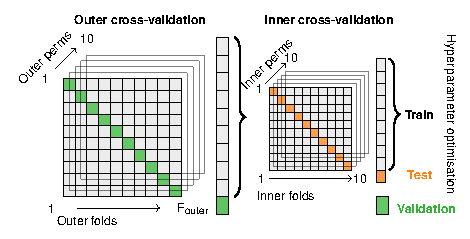
\includegraphics[width=0.24\textwidth]{ncv.pdf}};








\end{tikzpicture}